\documentclass[12pt]{article}
\usepackage{amsthm,amssymb,amsfonts,amsmath,amstext,systeme}
\usepackage{graphicx,float}
\usepackage{tabularx}

\marginparwidth 0pt
\oddsidemargin -1.2 truecm
\evensidemargin  0pt 
\marginparsep 0pt
\topmargin -2.2truecm
\linespread{1}
\textheight 25.8 truecm
\textwidth 18.5 truecm
\newenvironment{remark}{\noindent{\bf Remark }}{\vspace{0mm}}
\newenvironment{remarks}{\noindent{\bf Remarks }}{\vspace{0mm}}
\newenvironment{question}{\noindent{\bf Question }}{\vspace{0mm}}
\newenvironment{questions}{\noindent{\bf Questions }}{\vspace{0mm}}
\newenvironment{note}{\noindent{\bf Note }}{\vspace{0mm}}
\newenvironment{summary}{\noindent{\bf Summary }}{\vspace{0mm}}
\newenvironment{back}{\noindent{\bf Background}}{\vspace{0mm}}
\newenvironment{conclude}{\noindent{\bf Conclusion}}{\vspace{0mm}}
\newenvironment{concludes}{\noindent{\bf Conclusions}}{\vspace{0mm}}
\newenvironment{dill}{\noindent{\bf Description of Dill's model}}{\vspace{0mm}}
\newenvironment{maths}{\noindent{\bf Mathematics needed}}{\vspace{0mm}}
\newenvironment{inst}{\noindent{\bf Instructions}}{\vspace{0mm}}
\newenvironment{notes}{\noindent{\bf Notes }}{\vspace{0mm}}
\newenvironment{theorem}{\noindent{\bf Theorem }}{\vspace{0mm}}
\newenvironment{example}{\noindent{\bf Example }}{\vspace{0mm}}
\newenvironment{examples}{\noindent{\bf Examples }}{\vspace{0mm}}
\newenvironment{topics}{\noindent{\bf Topics}}{\vspace{0mm}}
\newenvironment{outcomes}{\noindent{\bf Expected Learning Outcomes}}{\vspace{0mm}}
\newenvironment{lemma}{\noindent{\bf Lemma }}{\vspace{0mm}}
\newenvironment{solution}{\noindent{\it Solution}}{\vspace{2mm}}
\newcommand{\ds}{\displaystyle}
\newcommand{\un}{\underline}
\newcommand{\bs}{\boldsymbol}

\begin{document}

\baselineskip 18 pt
\begin{center}
	{\large \bf HKDSE MATH CORE 2023 Past Paper I}\\
	\vspace{2 mm}

\end{center}
\vspace{0.05cm}

\begin{enumerate}
	\item \textbf{HKDSE MATH CORE 2023 Past Paper I Q1}\\
	Make $h$ the subject of the formula $\dfrac{5}{h + k} = \dfrac{k}{h - 3}$. \\(3 marks)

	\item \textbf{HKDSE MATH CORE 2023 Past Paper I Q2}\\
	Simplify $\dfrac{x^{-8}y}{(x^7y^9)^{-6}}$ and express your answer with positive indices. \\(3 marks)	

	\item \textbf{HKDSE MATH CORE 2023 Past Paper I Q3}\\
	A packet of cheese is termed regular if its weight is measured as 220 g correct to the nearest 10 g. Someone claims that the total weight of 250 regular packets of cheese can be measured as 53.6 kg
	correct to the nearest 0.1 kg. Is the claim correct? Explain your answer. \\(3 marks)

	\item \textbf{HKDSE MATH CORE 2023 Past Paper I Q4}\\
	Consider the compound inequality $$3x + 2 > \dfrac{4x - 5}{2} \text{ and } 3x - 2 < 7 \dots\dots\dots\dots\dots (*) .$$
	\begin{enumerate}
		\item[(a)] Solve $(*)$.
		\item[(b)] How many negative integers satisfy $(*)$?
	\end{enumerate}
	(4 marks)

	\item \textbf{HKDSE MATH CORE 2023 Past Paper I Q5}\\
	On a ferry, the number of female passengers is 40\% more than the number of male passengers. If 24 female passengers leave the ferry, then the number of male passengers is 40\% more than the number of female passengers. Find the number of male passengers on the ferry.  \\(4 marks)


	\item \textbf{HKDSE MATH CORE 2023 Past Paper I Q6}\\
	Let $a$, $b$ and $c$ be non-zero numbers such that $7a = 6b$ and $\dfrac{4a - 3c}{2b - c} = 9$. Find
	\begin{enumerate}
		\item[(a)] $a : b : c$,
		\item[(b)] $\dfrac{5a + 8b}{7b + 3c}$.
	\end{enumerate}
	(4 marks)

	\item \textbf{HKDSE MATH CORE 2023 Past Paper I Q7}\\
	In Figure 1, $PR$ is a diameter of the circle $PQRS$. Denote the point of intersection of $PR$ and $QS$ by $T$.
	\begin{figure}[H]
		\centering
		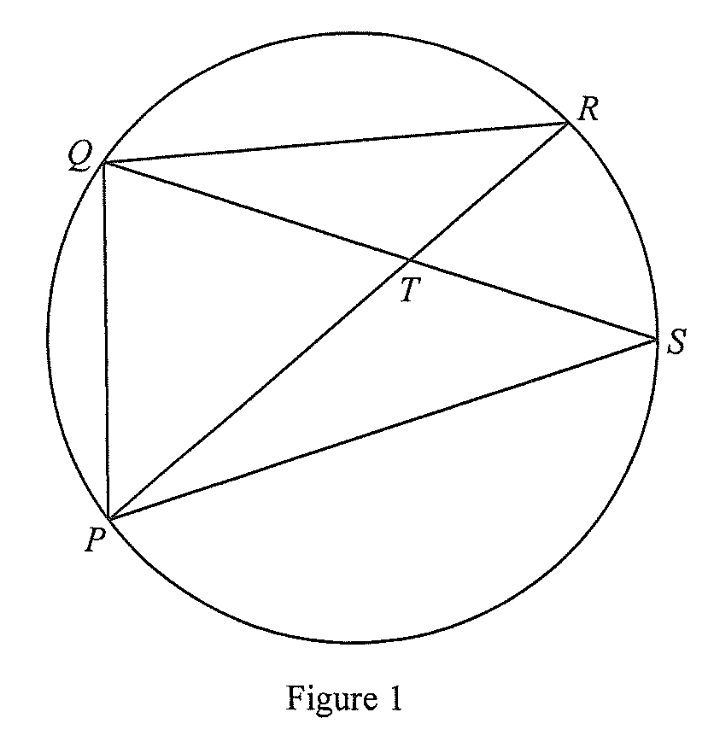
\includegraphics[width = .3\linewidth]{2023Figure1.1}
	\end{figure}
	If $\angle PSQ = 41^\circ$ and $\angle PTQ = 68^\circ$, find $\angle RQS$ and $\angle PQS$. \\(4 marks)
	
	\item \textbf{HKDSE MATH CORE 2023 Past Paper I Q8}\\
	In Figure 2, $AB$ and $CD$ intersect at the point $E$. It is given that $AC // DB$.
	\begin{figure}[H]
		\centering
		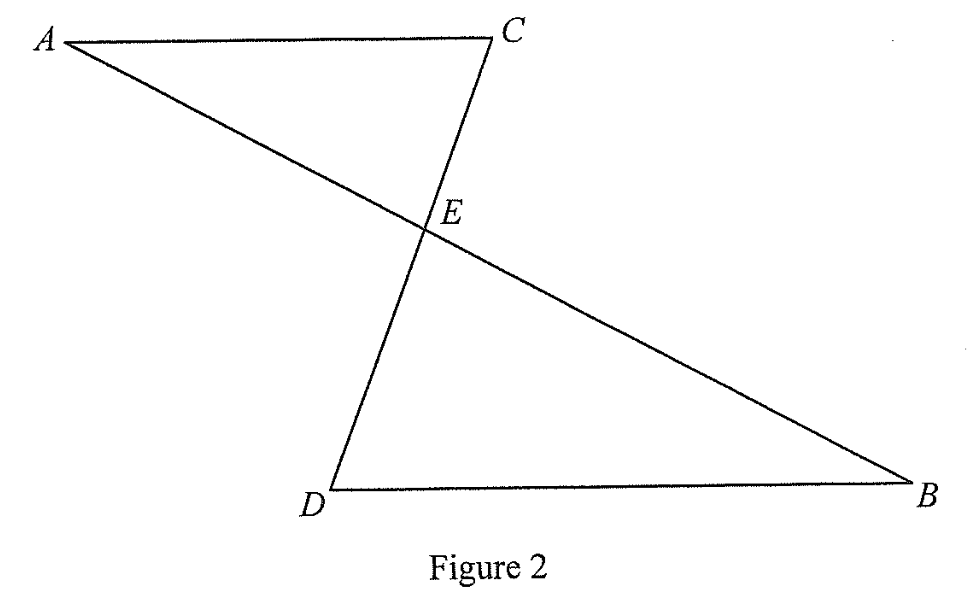
\includegraphics[width = .3\linewidth]{2023Figure1.2}
	\end{figure}
	\begin{enumerate}
		\item[(a)] Prove that $\triangle ACE \sim \triangle BDE$.
		\item[(b)] Suppose that $AB = 20$ cm, $AC = 10$ cm and $CE = 7$ cm. Is $\triangle BDE$ is a right-angled triangle? Explain your answer.
	\end{enumerate}
	(5 marks)

	\item \textbf{HKDSE MATH CORE 2023 Past Paper I Q9}\\
	The stem-and-leaf diagram below shoes the distribution of the numbers of working hours of a group of workers in a week.
	\begin{table}[htbp]
		\centering
		\begin{tabular}{r|l@{\hspace{4 pt}}}
		   Stem (tens) & Leaf (units)     \\
			\hline
			2     & $a$ 5 5 6 6 8 8\\    
			3     & 3 3 3 4 5 5 9 9\\    
			4     & 0 1 4 4 5 6 7 7 9\\    
		\end{tabular}
		\label{tab:addlabel}
	\end{table}
	The range of the distribution is 27.
	\begin{enumerate}
		\item[(a)] Find the mean and the mode of the distribution.
		\item[(b)] If a worker is randomly selected from the group, find the probability that the number of working hours of the selected worker in the week exceeds the mode of the distribution.
	\end{enumerate}
	(5 marks)

	\item \textbf{HKDSE MATH CORE 2023 Past Paper I Q10}\\
	It is given that $A$ and $B$ are two distinct points in a rectangular coordinate plane. Let $P$ be a moving point in the rectangular coordinate plane such that $P$ is equidistant from $A$ and $B$. Denote the locus of $P$ by $\Gamma$.
	\begin{enumerate}
		\item[(a)] Describe the grometric relationship between $\Gamma$ and $AB$. \\(1 marks)
		\item[(b)] Suppose that the coordinates of $A$ are $(2, -4)$ and the equation of $\Gamma$ is $3x + y - 12 = 0$. Find 
		\begin{enumerate}
			\item[(i)] the equation of the straight line which passes through $A$ and $B$,
			\item[(ii)] the equation of the circle with $AB$ as a diameter.
		\end{enumerate}
		(5 marks)
	\end{enumerate}

	\item \textbf{HKDSE MATH CORE 2023 Past Paper I Q11}\\
	The table below shoes the distribution of the numbers of calculators owned by a class of students.
	$$\begin{array}{|c|c|c|c|c|}
		\hline
		\text{Number of calculators owned} & 1 & 2 & 3 & 4 \\
		\hline
		\text{Number of student} & 8 & 5 & n & 1 \\
		\hline
	\end{array}$$
	The mean of the distribution is 2.
	\begin{enumerate}
		\item[(a)] Find the median, inter-quatile range and the variance of the above distribution. \\(5 marks)
		\item[(b)] Two students now withdraw from the class. It is found that the mean of the distribution remains unchanged. Is there any change in the range of the distribution due to the withdrawal of the two students? Explain your answer. \\(2 marks)
	\end{enumerate}

	\item \textbf{HKDSE MATH CORE 2023 Past Paper I Q12}\\
	It is given that $f(x)$ is partly constant and partly varies as $x^2$. Suppose that $f(10) = 62$ and $f(15) = 122$.
	\begin{enumerate}
		\item[(a)] Find $f(5)$. \\(3 marks)
		\item[(b)] Suppose that $U(0, u)$ and $V(5,v)$ are points lying on the graph of $y = f(x)$. The horizontal line passing through $V$ cuts the $y$-axis at the point $W$. Denote the circle which passes through $U$, $V$ and $W$ by $C$. Express the circumference of $C$ in terms of $\pi$. \\(4 marks)
	\end{enumerate}

	\item \textbf{HKDSE MATH CORE 2023 Past Paper I Q13}\\
	Define $g(x) = x^3 + 5x^2 - 12x - 1$. Let $h(x) = 3x^4 + ax^3 - 16x + bx + c$, where $a$, $b$ and $c$ are constants. When $h(x)$ is divided by $g(x)$, the quotient and the remainder are equal.
	\begin{enumerate}
		\item[(a)] Find the quotient when $h(x)$ is divided by $g(x)$. \\(3 marks)
		\item[(b)] How many rational roots does the equation $h(x) = 0$ have? Explain your answer. \\(4 marks)
	\end{enumerate}

	\item \textbf{HKDSE MATH CORE 2023 Past Paper I Q14}\\
	The base radius and the curved area of a solid metal reight circular cone are 14 cm and $700\pi$ cm$^2$ respectively.
	\begin{enumerate}
		\item[(a)] Find the height of the circular cone. \\(3 marks)
		\item[(b)] The circular cone is divided into a right circular cone $X$ anda frustum $Y$ by a plane which is parallel to its base. The curve surface area of $Y$ is 15 times the curved surface area of $X$.
		\begin{enumerate}
			\item[(i)] Express the volume of $Y$ in terms of $\pi$.
			\item[(ii)] If $Y$ is melted and recast into 2 identical solid spheres, find the diameter of each sphere.
		\end{enumerate}
		(5 marks)
	\end{enumerate}

	\item \textbf{HKDSE MATH CORE 2023 Past Paper I Q15}\\
	In a box, there are 4 red balls and 4 black balls. From the box, 2 balls are randomly chosen at the same time.
	\begin{enumerate}
		\item[(a)] Find the probability that the 2 balls chosen are red. \\(2 marks)
		\item[(b)] In a bag, there are 8 red balls. The 2 balls form the box are put into the bag and then 3 balls are randomly chosen at the smae time from the bag. Find the probability tha tthe 3 balls chosen are of the same colour. \\(2 marks)
	\end{enumerate}

	\item \textbf{HKDSE MATH CORE 2023 Past Paper I Q16}
	\begin{enumerate}
		\item[(a)] Let $a$ and $b$ be real constants. If the roots of the equation $x^2 + ax + b = 0$ are $p$ and $5p$, prove that $5a^2 = 36b$. \\(2 marks)
		\item[(b)] Denote the circle $x^2 + y^2 - 6x - 12y + 20 = 0$ by $C$. Find the constant $m$ such that the straight line $y = mx$ cuts $C$ at the points $Q$ and $R$ with $OQ:QR = 1:4$, where $O$ is the origin. \\(3 marks)
	\end{enumerate}

	\item \textbf{HKDSE MATH CORE 2023 Past Paper I Q17}\\
	In a bag, there are 4 green pens, 7 blue pens and 8 black pens. If 5 pens are randomly drawn from the bag at the same time,
	\begin{enumerate}
		\item[(a)] find the probability that exactly 4 green pens are drawn; \\(2 marks)
		\item[(b)] find the probability that exactly 3 green pens are drawn; \\(2 marks)
		\item[(c)] find the probability that not more than 2 green pens are drawn. \\(2 marks)
	\end{enumerate}

	\item \textbf{HKDSE MATH CORE 2023 Past Paper I Q18}\\
	The equation of the parabola $\Gamma$ is $2x^2 - 2kx + 2x - 3k + 8$, where $k$ is a real constant. Denote the straight line $y = 19$ by $L$.
	\begin{enumerate}
		\item[(a)] Prove that $L$ and $\Gamma$ intersect at two distinct points. \\(3 marks)
		\item[(b)] The points of intersection of $L$ and $\Gamma$ are $A$ and $B$.
		\begin{enumerate}
			\item[(i)] Let $a$ and $b$ be the $x$-coordinates of $A$ and $B$ respectively. Prove that $(a - b)^2 = k^2 + 4k + 23$.
			\item[(ii)] Is it possible that the distance between $A$ and $B$ is less than 4? Explain your answer.
		\end{enumerate}
		(5 marks)
	\end{enumerate}

	\item \textbf{HKDSE MATH CORE 2023 Past Paper I Q19}\\
	$ABC$ is a thin triangular metal sheet, where $BC = 24$ cm, $\angle BAC = 30^\circ$ and $\angle ACB = 42^\circ$.	
	\begin{enumerate}
		\item[(a)] Find the length of $AC$. \\(2 marks)
		\item[(b)] In Figure 2, the thin metal sheet $ABC$ is held such that only the vertex $B$ lies on the horizontal ground. $D$ and $E$ are points lying on the horizontal ground vertically below vertices $A$ and $C$ respectively. $AC$ produced meets the horizontal ground at the point $F$. A craftman finds that $AD = 10$ cm and $CE = 2$ cm.
		\begin{figure}[H]
			\centering
			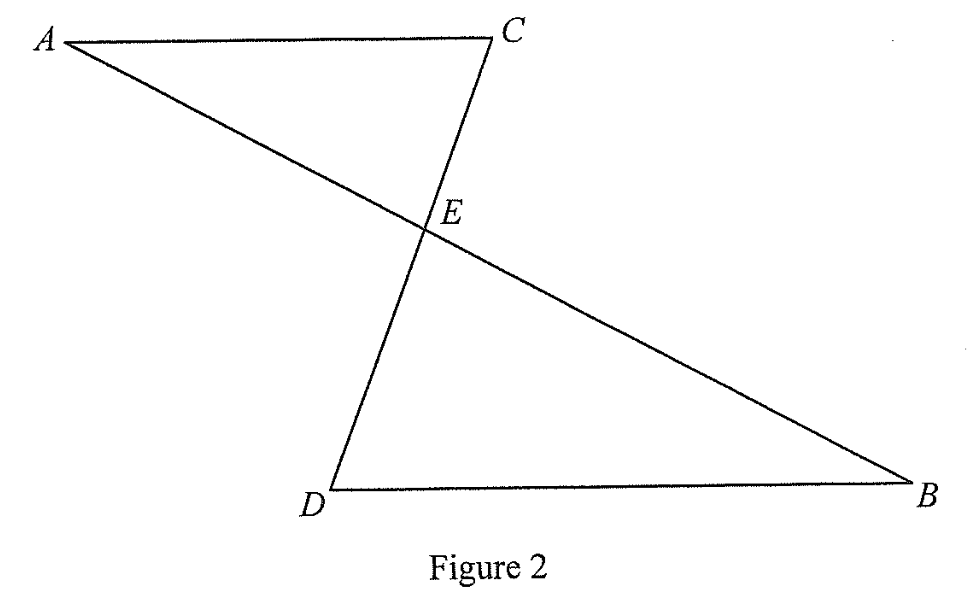
\includegraphics[width = .3\linewidth]{2023Figure1.2}
		\end{figure}
		\begin{enumerate}
			\item[(i)] Find the distance between $C$ and $F$.
			\item[(ii)] Find the area of $\triangle ABF$.
			\item[(ii)] Find the inclination of the thin metal sheet $ABC$ to the horizontal ground.
			\item[(ii)] The craftman claims that the area of $\triangle BDF$ is greater than 460 cm$^2$. Do you agree? Explain your answer.
		\end{enumerate}
		(11 marks)
	\end{enumerate}


\end{enumerate}
\end{document}